\documentclass[a4paper,14pt]{extarticle}

% ------ GLOBAL ------

\usepackage{calc,etoolbox,float,microtype,soul,xspace,textcomp,xltxtra}
\usepackage[table]{xcolor}

% ------ LANGUAGE ------

\usepackage{polyglossia}
\setdefaultlanguage[babelshorthands=true]{russian}
\setotherlanguage{english}
\defaultfontfeatures{Ligatures=TeX,Mapping=tex-text}

% ------ PAGE VIEW ------

\usepackage[left=2cm,right=2cm,top=3cm,bottom=4cm]{geometry}
\setmainfont[Ligatures=TeX]{Liberation Serif}
\setsansfont[Ligatures=TeX]{Liberation Sans}

% ------ HEADER & FOOTER ------

\usepackage{fancyhdr}
\pagestyle{fancy}
\fancyhead{}\renewcommand{\headrulewidth}{0mm}\fancyfoot[CE,CO]{\thepage}
\fancypagestyle{plain}{\fancyhead{}\renewcommand{\headrulewidth}{0mm}\fancyfoot{}}


\usepackage{graphicx}


\begin{document}
 
\section*{Supplementary Figure 1. Representative Hi-C maps for DNAse I Hi-C protocols}

\begin{figure}[hp!] \includegraphics[width=1\textwidth]{ma-pe_s30_ALL_535.pdf} \end{figure}

\begin{figure}[hp!] \includegraphics[width=1\textwidth]{ma-pe_s30_chr2_5kb_1.pdf} \end{figure}

\begin{figure}[hp!] \includegraphics[width=1\textwidth]{ma-pe_s30_chr2_25kb_2.pdf} \end{figure}

\begin{figure}[hp!] 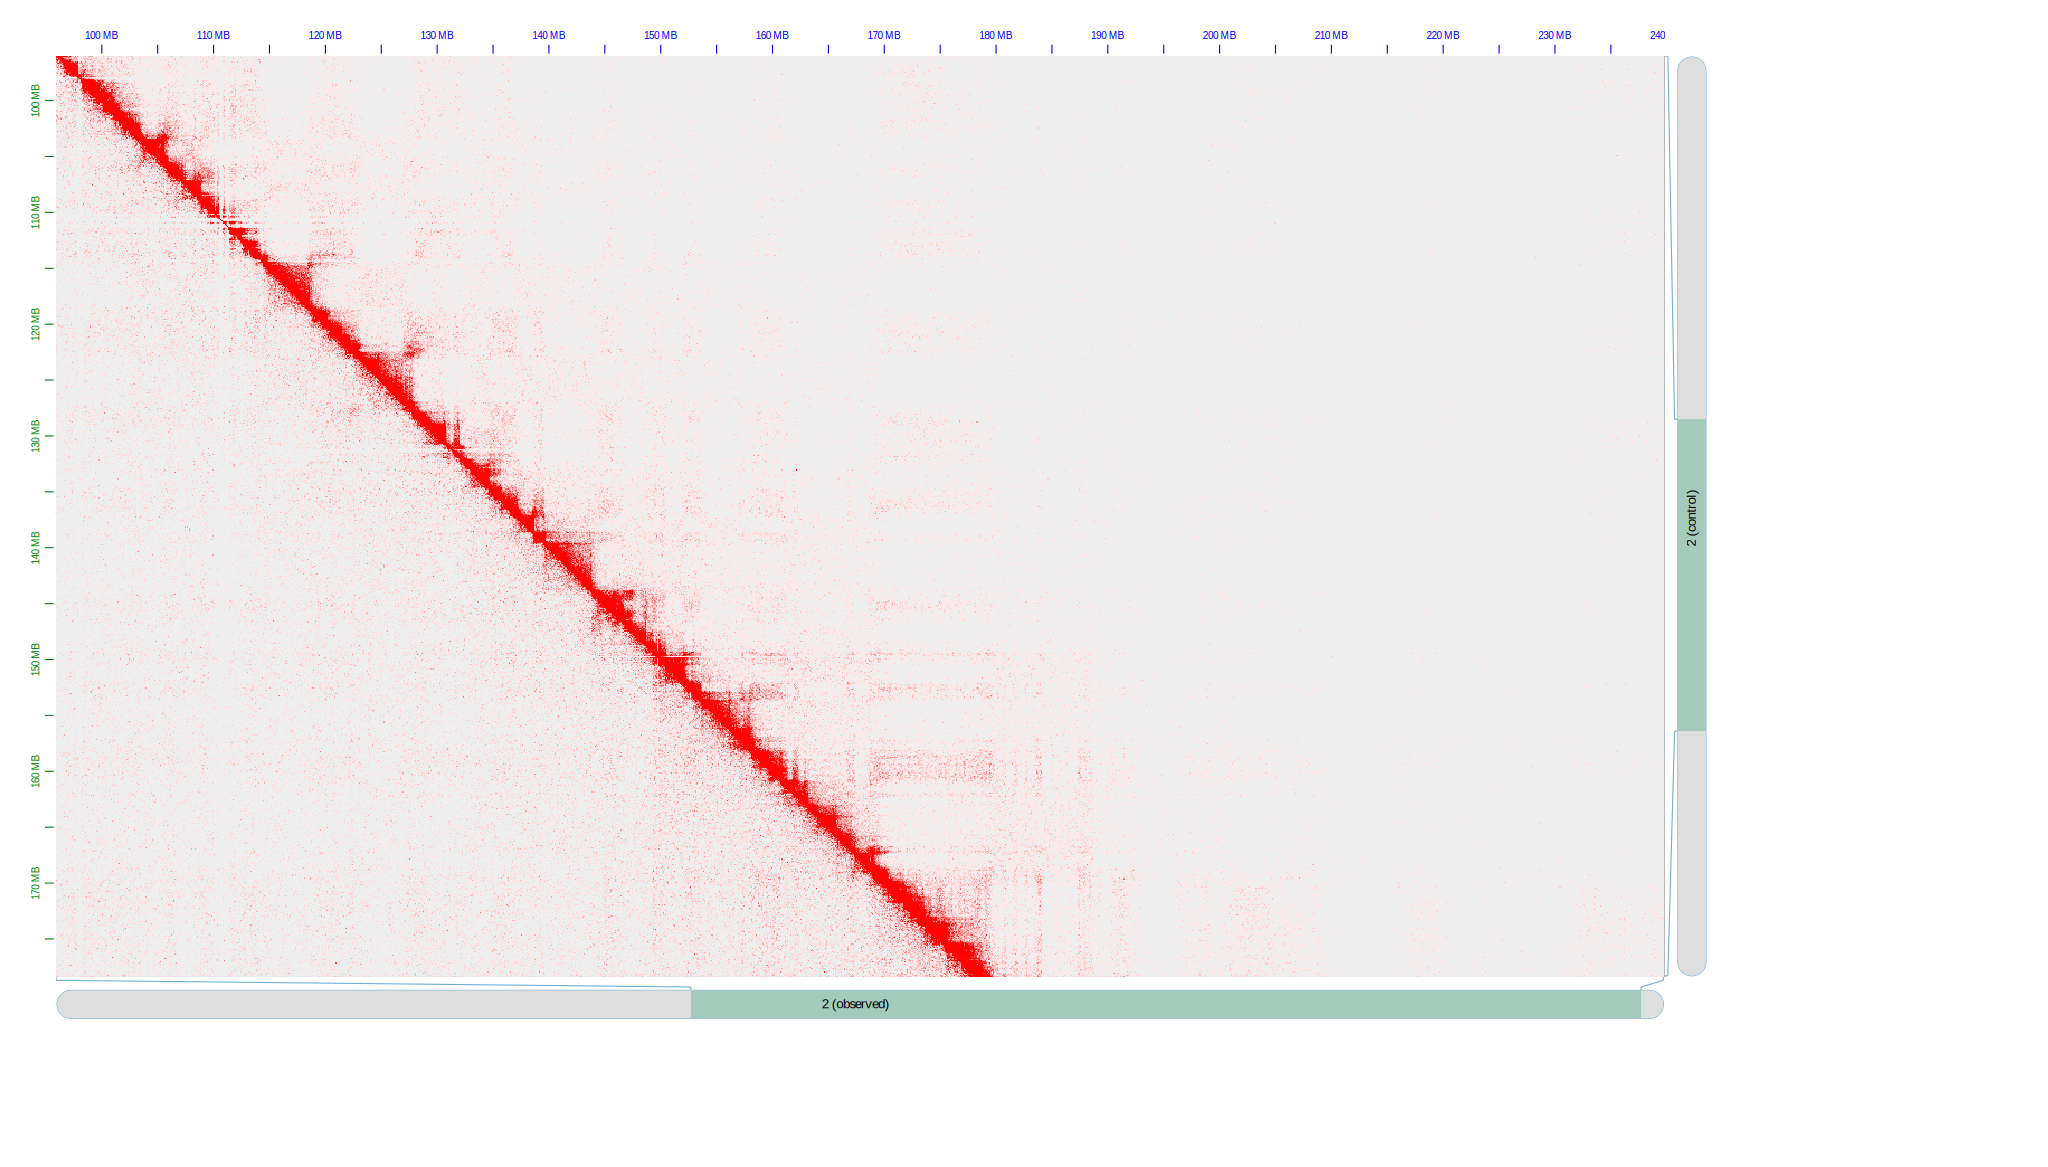
\includegraphics[width=1\textwidth]{ma-pe_s30_chr2_100kb_8.pdf} \end{figure}

\begin{figure}[hp!] \includegraphics[width=1\textwidth]{ma-pe_s30_chr2_500kb_30.pdf} \end{figure}

\begin{figure}[hp!] \includegraphics[width=1\textwidth]{ma-wgs_s30_ALL_366.pdf} \end{figure}

\begin{figure}[hp!] \includegraphics[width=1\textwidth]{ma-wgs_s30_chr4_5kb_0.pdf} \end{figure}

\begin{figure}[hp!] \includegraphics[width=1\textwidth]{ma-wgs_s30_chr4_25kb_1.pdf} \end{figure}

\begin{figure}[hp!] \includegraphics[width=1\textwidth]{ma-wgs_s30_chr4_100kb_9.pdf} \end{figure}

\begin{figure}[hp!] \includegraphics[width=1\textwidth]{ma-wgs_s30_chr4_500-100kb_13.pdf} \end{figure}

\begin{figure}[hp!] \includegraphics[width=1\textwidth]{ramani-brain_ALL_275.pdf} \end{figure}

\begin{figure}[hp!] 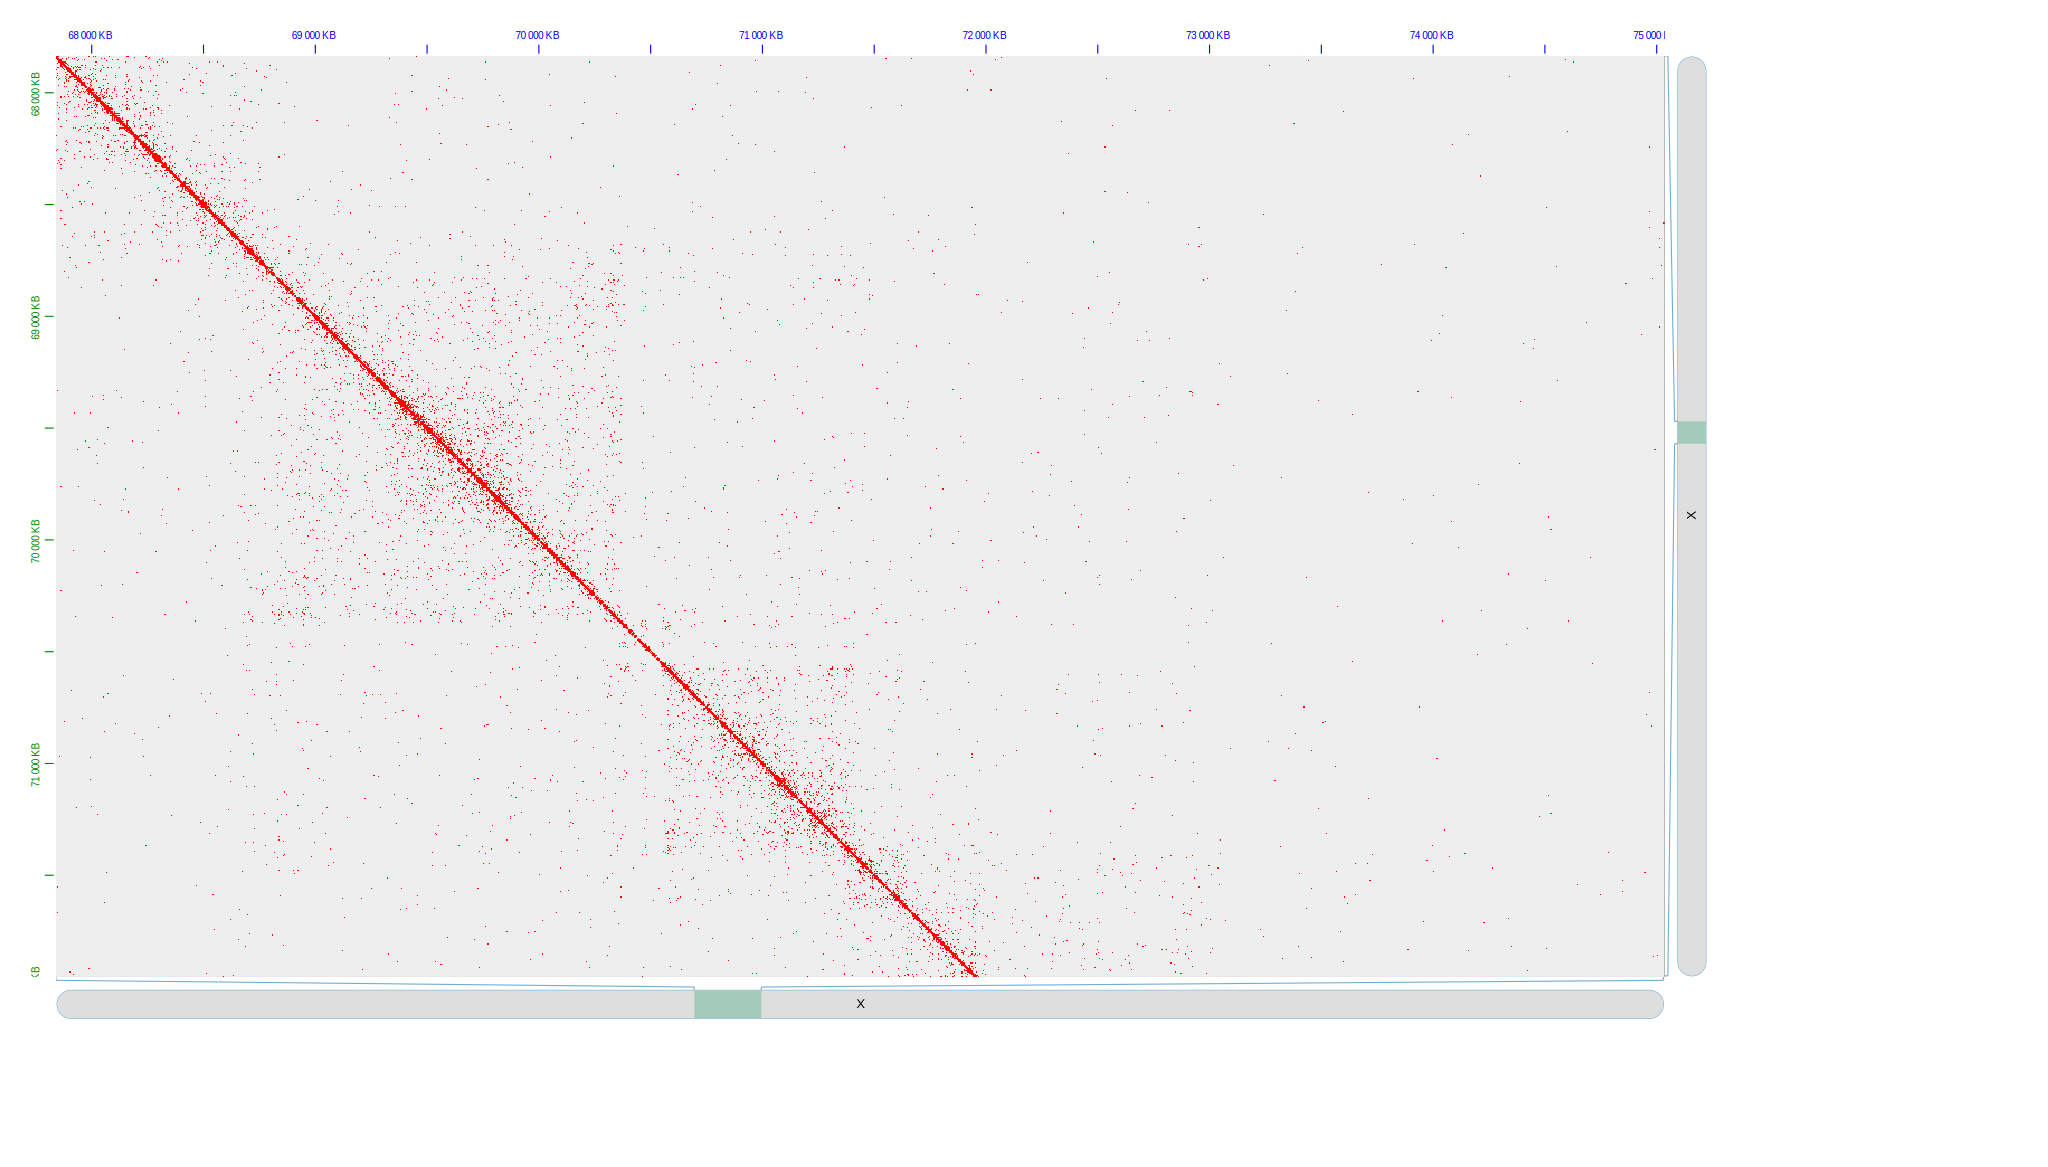
\includegraphics[width=1\textwidth]{ramani-brain_chrX_5kb_0.pdf} \end{figure}

\begin{figure}[hp!] \includegraphics[width=1\textwidth]{ramani-brain_chrX_25kb_1.pdf} \end{figure}

\begin{figure}[hp!] \includegraphics[width=1\textwidth]{ramani-brain_chrX_100kb_5.pdf} \end{figure}

\begin{figure}[hp!] \includegraphics[width=1\textwidth]{ramani-brain_chrX_500-100kb_7.pdf} \end{figure}

\begin{figure}[hp!] \includegraphics[width=1\textwidth]{s5_s30_ALL_376.pdf} \end{figure}

\begin{figure}[hp!] \includegraphics[width=1\textwidth]{s5_s30_chr5_5kb_0.pdf} \end{figure}

\begin{figure}[hp!] \includegraphics[width=1\textwidth]{s5_s30_chr5_25kb_3.pdf} \end{figure}

\begin{figure}[hp!] \includegraphics[width=1\textwidth]{s5_s30_chr5_100kb_14.pdf} \end{figure}

\begin{figure}[hp!] \includegraphics[width=1\textwidth]{s5_s30_chr5_500-100kb_14.pdf} \end{figure}

\end{document}
